



\title{Solana: Una nuova architettura per una blockchain ad alte prestazioni  v0.8.14 }

\author{
        Anatoly Yakovenko \\
        anatoly@solana.io\\
}
\date{}

\documentclass[12pt]{article}

% \usepackage{draftwatermark}
% \SetWatermarkText{Confidential}
% \SetWatermarkScale{5}
% \SetWatermarkColor[gray]{0.95}

\usepackage{graphicx}
\usepackage{bytefield}
\usepackage{makecell}
\usepackage[utf8]{inputenc}


\usepackage[]{hyperref}
\hypersetup{
    pdftitle={Solana:  Una nuova architettura per una blockchain ad alte prestazioni},
    pdfauthor={anatoly@solana.io},
    pdfsubject={blockchain},
    pdfkeywords={blockchain, bitcoin, cryptocurrency},
    bookmarksnumbered=true,
    bookmarksopen=true,
    bookmarksopenlevel=1,
    colorlinks=true,
    pdfstartview=Fit,
    pdfpagemode=UseOutlines,    % this is the option you were lookin for
    pdfpagelayout=TwoPageRight
}

\begin{document}
\maketitle

\textbf{\footnotesize Esonero Legale}\scriptsize
~~Nulla nel presente White Paper è un'offerta di vendita o un modo per indurre all' acquisto di token. Solana pubblica questo White Paper esclusivamente per ricevere feedback e commenti da parte del pubblico. Se e quando Solana metterà in vendita dei token (o un semplice accordo per token futuri), lo farà attraverso documenti di offerta definitivi, tra cui un documento informativo e fattori di rischio. Si prevede che tali documenti definitivi comprenderanno anche una versione aggiornata del White Paper, che potrebbe differire in misura significativa dalla versione attuale. Se e quando Solana farà tale offerta negli Stati Uniti, l'offerta sarà probabilmente disponibile solo per gli investitori accreditati.


Nessun elemento del presente White Paper deve essere trattato o letto come una garanzia o una promessa di come si svilupperanno le attività di Solana  o dell'utilità o del valore dei gettoni o di come essi verranno distribuiti. Il presente White Paper delinea i piani attuali, che potrebbero cambiare a discrezione di Solana e il cui successo dipenderà da molti fattori al di fuori del controllo di Solana, tra cui i fattori di mercato e i fattori nel settore dei dati e della industria delle cryptovalute. Qualsiasi dichiarazione su eventi futuri si basa esclusivamente sull'analisi delle questioni descritte nel presente White Paper effettuata da Solana. Tale analisi potrebbe rivelarsi errata.


\begin{abstract}\label{Astratto}
Il presente documento propone una nuova architettura blockchain basata sulla Proof of History (PoH) - una prova per verificare l'ordine e il passaggio del tempo tra gli eventi. PoH è usato per codificare il passaggio sicuro del tempo in un libro mastro - una struttura di dati solo append. Se utilizzato insieme a un algoritmo di consenso come il Proof of Work (PoW) o il Proof of Stake (PoS), il PoH può ridurre l'overhead in un di messaggistica in una macchina a stato replicato Byzantine Fault Tolerant, con tempi di finalizzazione inferiori ai secondi. Questo articolo propone anche due algoritmi che sfruttano le proprietà di conservazione del tempo del registro PoH - un algoritmo PoS che può recuperare da partizioni di qualsiasi dimensione e un efficiente streaming Proof of Replication (PoRep). La combinazione di PoRep e PoH fornisce una difesa contro la falsificazione del libro mastro per quanto riguarda il tempo (ordinamento) e la conservazione. Il protocollo viene analizzato su una rete da $1$~gbps e questo articolo mostra che con l'hardware odierno è possibile effettuare transazioni fino a $710$k al secondo.

\end{abstract}


\section{Introduzione}\normalsize
Blockchain è l'implementazione di una macchina a stato replicato con tolleranza ai guasti. Le blockchain attualmente disponibili al pubblico non si basano sul tempo, o fanno un'ipotesi debole sulle capacità del partecipante di mantenere il tempo~\cite{tendermint,hashgraph}. Ogni nodo della rete di solito si basa sul proprio orologio locale senza che gli altri partecipanti ne siano a conoscenza. La mancanza di una fonte di tempo affidabile significa che quando un messaggio viene utilizzato per accettare o rifiutare un messaggio, non vi è alcuna garanzia che ogni altro partecipante alla rete effettuerà la stessa scelta. Il PoH qui presentato è stato progettato per creare un registro con un passaggio di tempo verificabile, cioè la durata tra gli eventi e l'ordinazione dei messaggi. Si prevede che ogni nodo della rete potrà contare sul passaggio del tempo registrato nel libro mastro senza doversi fidare di terze parti.

\section{Indice}
Il resto di questo articolo è organizzato come segue. La progettazione generale del sistema è descritta nella Sezione ~\ref{design}. Una descrizione dettagliata della Proof of History è descritta nella Sezione ~\ref{proof_of_history}. Una descrizione dettagliata dell'algoritmo Proof of Stake proposto per la verifica del consenso  è descritta nella sezione~\ref{proof_of_stake}. Una descrizione dettagliata della fast Proof of Replication  è descritta nella Sezione ~\ref{porep}. L'architettura di sistema e i limiti delle prestazioni sono analizzati nella Sezione ~\ref{architettura_di_sistema}. Un motore a contratto intelligente ad alte prestazioni e facile da usare per le GPU è descritto nella Sezione ~\ref{sec:smartcontracts}.

\section{Network Design}\label{design}

\begin{figure}[h]
  \begin{center}
    \centering
    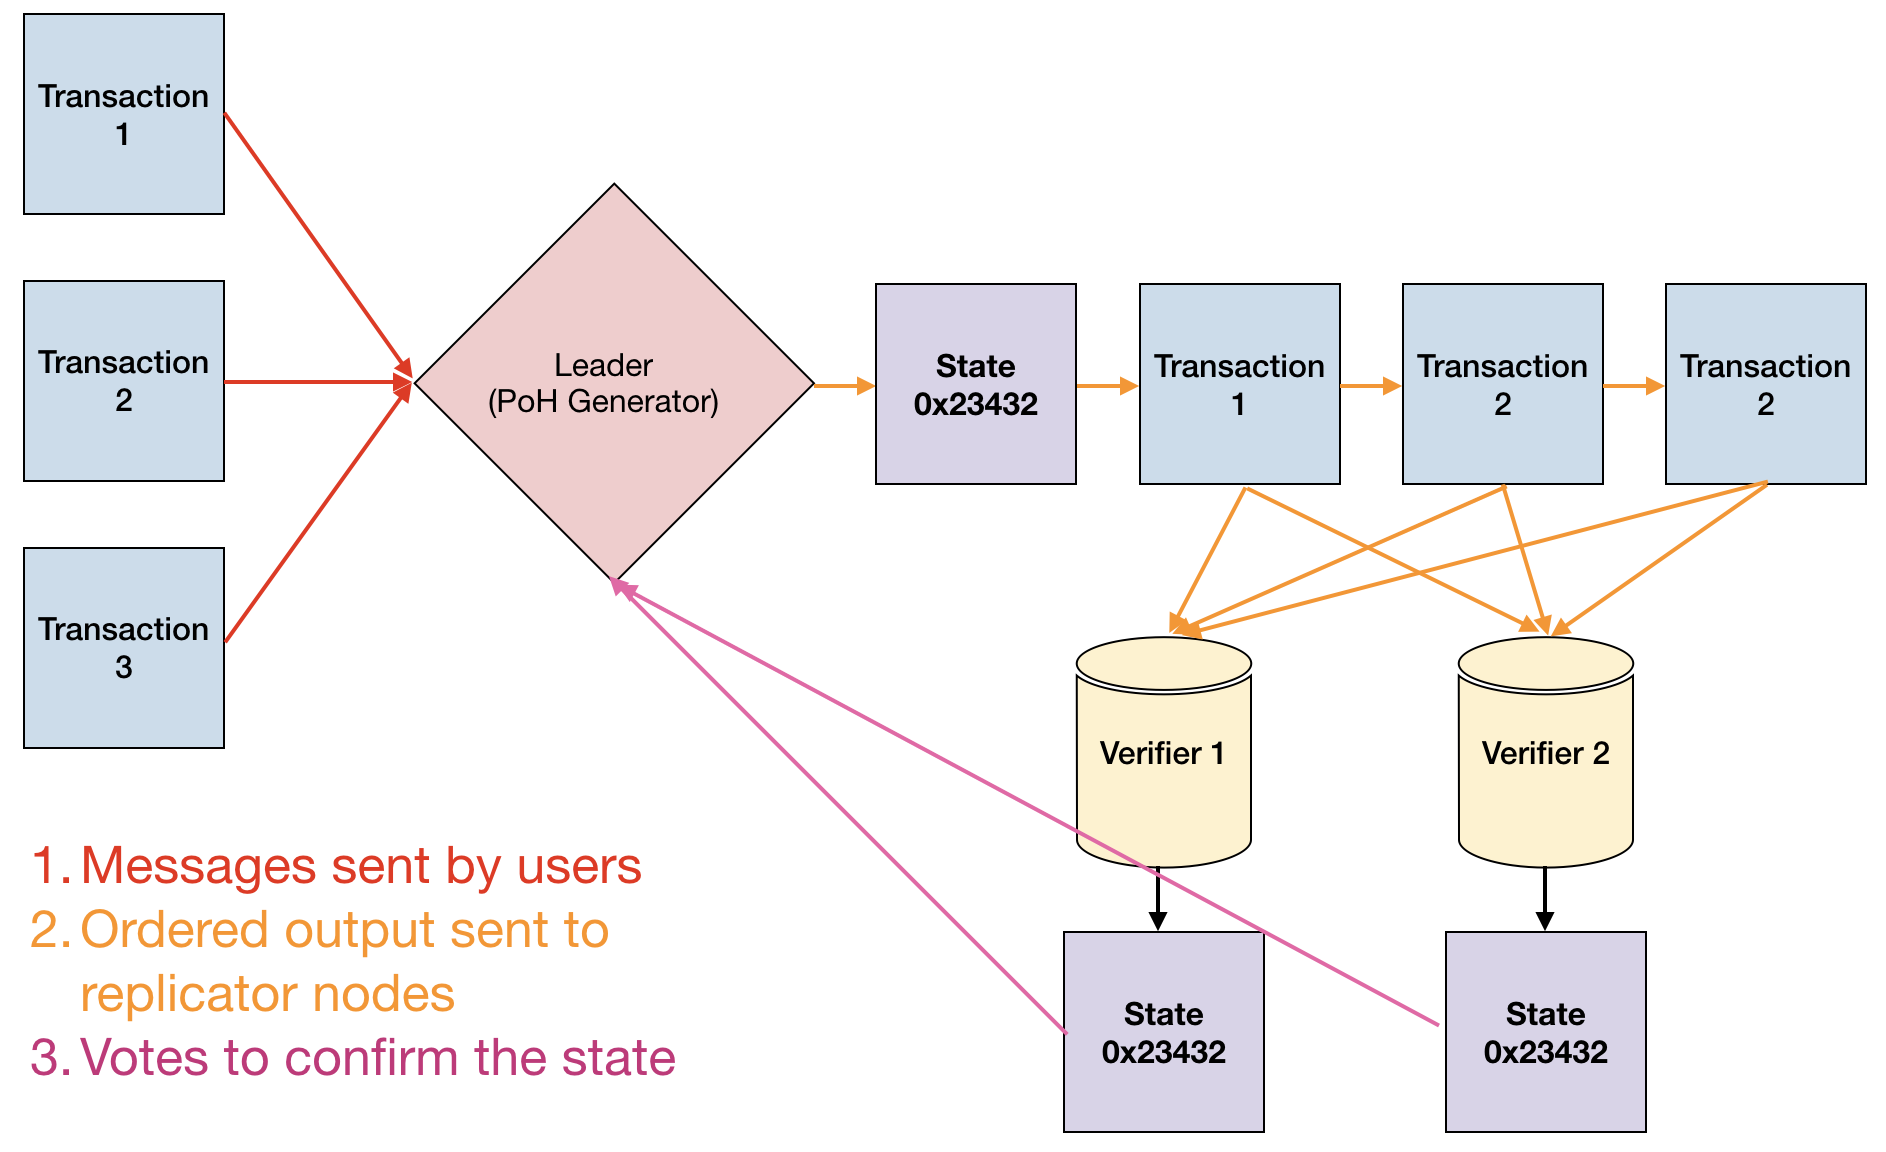
\includegraphics[width=\textwidth]{figures/network_design_001.png}
    \caption[Fig 1]{Transazioni attraverso la rete.\label{fig:design}}
  \end{center}
  \end{figure}

Come mostrato nella Figura~\ref{fig:design}, in qualsiasi momento un nodo di sistema è designato come Leader per generare una sequenza di Proof of History, fornendo alla rete una coerenza di lettura globale e un passaggio del tempo verificabile. Il Leader sequenzia i messaggi degli utenti e li ordina in modo tale che possano essere elaborati in modo efficiente da altri nodi del sistema, massimizzando la produttività. Il Leader esegue le transazioni sullo stato corrente memorizzato nella RAM e pubblica le transazioni e una firma dello stato finale sui nodi di replica chiamati Verificatori. I Verificatori eseguono le stesse operazioni sulle loro copie dello stato e pubblicano le loro firme calcolate dello stato come conferme. Le conferme pubblicate servono come voti per l'algoritmo di consenso.

In uno stato non partizionato, in qualsiasi momento, c'è un Leader nella rete. Ciascun nodo verificatore ha le stesse capacità hardware di un Leader e può essere eletto Leader, questo avviene tramite elezioni basate su PdS. Le elezioni per l'algoritmo di PdS proposto sono trattate in modo approfondito nella Sezione~\ref{subsec:elections}.

Per il di teorema CAP, la Coerenza è quasi sempre scelta rispetto alla Disponibilità in caso di Partizione. Nel caso di una partizione di grandi dimensioni, questo documento propone un meccanismo per ripristinare il controllo della rete da una partizione di qualsiasi dimensione. Questo è trattato in modo approfondito nella Sezione~\ref{availability}.	

\section{Proof of History}\label{proof_of_history}

La Proof of History è una sequenza di calcolo che può fornire un modo per verificare crittograficamente il passaggio del tempo tra due eventi. Utilizza una funzione di sicurezza crittografica scritta in modo che non sia possibile prevedere l'uscita dall'ingresso e che debba essere eseguita completamente per generare l'uscita. La funzione viene eseguita in sequenza su un singolo core, la cui uscita precedente è l'ingresso corrente, registrando periodicamente l'uscita corrente e quante volte è stata richiamata. L'uscita può quindi essere ricalcolata e verificata da computer esterni in parallelo controllando ogni segmento di sequenza su un nucleo separato.

I dati possono essere timestampati in questa sequenza aggiungendo i dati (o un hash di alcuni dati) nello stato della funzione. La registrazione dello stato, dell'indice e dei dati così come sono stati aggiunti alle sequenze fornisce una timestamp in grado di garantire che i dati siano stati creati in un momento precedente alla generazione dell'hash successivo nella sequenza. Questo design supporta anche l'horizontal scaling, in quanto più generatori possono sincronizzarsi tra loro mescolando il loro stato nelle sequenze degli altri. L'horizontal scaling è discusso in modo approfondito nella Sezione~\ref{poh:scale}\\

\subsection{Description}
Il sistema è progettato per funzionare come segue. Con una funzione hash crittografica, il cui output non può essere previsto senza eseguire la funzione (ad esempio \texttt{sha256}, \texttt{ripemd}, ecc.), eseguire la funzione da un valore iniziale casuale e prenderne l'output e passarlo nuovamente come ingresso nella stessa funzione. Registrare il numero di volte che la funzione è stata richiamata e l'uscita ad ogni chiamata. Il valore casuale di partenza scelto potrebbe essere qualsiasi stringa, come la prima pagina del New York Times di quel giorno.
\\\\
\noindent Per esempio: \noindent
\begin{center}
  \begin{tabular}{  l  l  r }
%    \hline
    \multicolumn{3}{c}{Sequenza PoH} \\
    \hline
    Index  & Operation & Output Hash \\ \hline
    $1$ & sha256(\char`\"any random starting value\char`\") & \texttt{hash1}\\ %\hline
    $2$ &  sha256(\texttt{hash1}) & \texttt{hash2}\\ %\hline
    $3$ & sha256(\texttt{hash2}) & \texttt{hash3}\\ %\hline
    \end{tabular}
\end{center}

\noindent Dove \texttt{hashN} rappresenta l'attuale outtup dell'hash.\\

È solo necessario pubblicare un subset degli hashes e degli indici ad un intervallo.\\

\noindent Per esempio:\\\\\noindent
\begin{center}
  \begin{tabular}{ l  l  r }
    \multicolumn{3}{c}{PoH Sequence} \\
    \hline
    Index & Operation & Output Hash \\ \hline
    $1$ & sha256(\char`\"any random starting value\char`\") & \texttt{hash1}\\
    $200$ &  sha256(\texttt{hash199}) & \texttt{hash200}\\
    $300$ & sha256(\texttt{hash299}) & \texttt{hash300} \\
    \end{tabular}
\end{center}

Finché la funzione hash scelta è resistente alle collisioni, questa serie di hash può essere calcolata in sequenza solo da un singolo thread del computer. Questo deriva dal fatto che non c'è modo di prevedere quale sarà il valore hash dell'indice $300$ senza eseguire l'algoritmo a partire dal valore iniziale $300$ volte. Così possiamo dedurre dalla struttura dei dati che del tempo reale è passato tra l'indice $0$ e l'indice $300$.

Nell'esempio in Figura~\ref{fig:poh_seq}, l'hash \texttt{62f51643c1} è stato prodotto contando fino a $510144806912$ e l'hash \texttt{c43d862d88} è stato prodotto contando fino a $510146904064$. Seguendo le proprietà precedentemente discusse dell'algoritmo PoH, possiamo fidarci che sia passato tempo reale tra il conteggio $510144806912$ e il conteggio $510146904064$.

\begin{figure}[h]
  \begin{center}
    \centering
    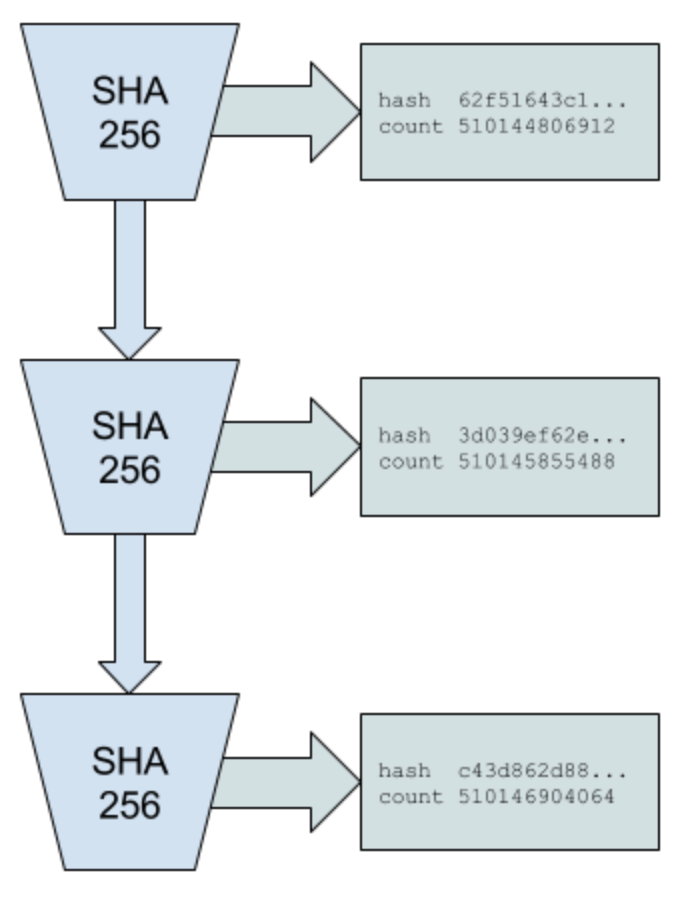
\includegraphics[width=0.5\textwidth]{figures/poh_sequence_001.png}
    \caption[Figure 2]{Sequenza Proof of History\label{fig:poh_seq}}
  \end{center}
  \end{figure}

\subsection{Timestamp for Events}

La sequenza di hash può anche essere usata per registrare che alcuni dati sono stati creati prima che fosse generato un particolare indice hash utilizzando una funzione "combina" per combinare il dato con l'hash corrente nell'indice corrente. I dati possono essere un hash crittograficamente univoco di dati di eventi arbitrari. La funzione combina può essere una semplice aggiunta di dati, o qualsiasi operazione che sia resistente alle collisioni. L'hash successivo generato rappresenta un timestamp dei dati, perché avrebbe potuto essere generato solo dopo l'inserimento di quel dato specifico.\\

\noindent Ad Esempio:\\\\\noindent
\begin{center}
  \begin{tabular}{ l l r }
    \multicolumn{3}{c}{PoH Sequence} \\
    \hline
    Index  & Operation  & Output Hash\\ \hline
    $1$ & sha256(\char`\"any random starting value\char`\") & \texttt{hash1}\\
    $200$ & sha256(\texttt{hash199}) & \texttt{hash200}\\
    $300$ & sha256(\texttt{hash299}) & \texttt{hash300}\\
    \end{tabular}
\end{center}


	\noindent Si verifica qualche evento esterno, come scattare una foto, oppure
	vengono creati dati digitali arbitrari:\\\\\noindent
\begin{center}
  \begin{tabular}{ l l r}
    \multicolumn{3}{c}{PoH Sequence With Data} \\
    \hline
    Index  & Operation & Output Hash\\ \hline
    $1$ & sha256(\char`\"any random starting value\char`\") & \texttt{hash1} \\
    $200$ & sha256(\texttt{hash199}) & \texttt{hash200} \\
    $300$  & sha256(\texttt{hash299}) & \texttt{hash300}\\
    $336$ & sha256(append(\texttt{hash335}, photograph\_sha256)) & \texttt{hash336}\\
    \end{tabular}
\end{center}


\texttt{Hash336} è calcolato a partire dai dati binari allegati di
\texttt{hash335} e il \texttt{sha256} della fotografia. L'indice
e il \texttt{sha256} della fotografia sono registrati come parte del file 
uscito in sequenza. Chiunque verifichi questa sequenza può quindi ricreare
questa modifica alla sequenza. La verifica può ancora essere effettuata in
parallelo ed è discusso nella Sezione ~\ref{poh:verify}

Poiché il processo iniziale è ancora sequenziale, possiamo dire che le cose inserite nella sequenza devono essersi verificate prima che il futuro valore fosse calcolato.

\begin{center}
  \begin{table}
  \begin{tabular}{l l r}
    \multicolumn{3}{c}{POH Sequence} \\ \hline
    Index & Operation & Output Hash \\ \hline
    $1$ & sha256(\char`\"any random starting value\char`\") & \texttt{hash1} \\
    $200$ & sha256(hash199) & \texttt{hash200} \\
    $300$ & sha256(hash299) & \texttt{hash300} \\
    $336$ & sha256(append(hash335, photograph1\_sha256)) & \texttt{hash336}\\
    $400$ & sha256(hash399) & \texttt{hash400} \\
    $500$ & sha256(hash499) & \texttt{hash500}\\
    $600$ & sha256(append(hash599, photograph2\_sha256)) & \texttt{hash600}\\
    $700$ & sha256(hash699) & \texttt{hash700}\\
    \end{tabular}
    \caption[Tabella 1]{Sequenza PoH con 2 eventi\label{table:multievent}}
    \end{table}
\end{center}

Nella sequenza rappresentata da Table~\ref{table:multievent}, \texttt{photograph2} è stato creato prima di \texttt{hash600}, e
\texttt{foto1} è stato creato prima di \texttt{hash336}. L'inserimento dei dati nella sequenza degli hash comporta la modifica di tutti i valori successivi della sequenza. Finché la funzione hash utilizzata è resistente alle collisioni e i dati sono stati aggiunti, dovrebbe essere impossibile calcolare in anticipo le sequenze future sulla base di una conoscenza preliminare dei dati che saranno integrati nella sequenza.\\

I dati che vengono mixati nella sequenza possono essere i dati grezzi stessi, o semplicemente un hash dei dati con i metadati di accompagnamento.\\

\begin{figure}[h]
  \begin{center}
    \centering
    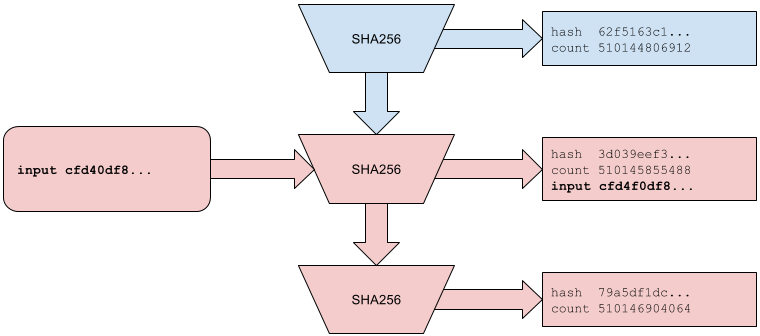
\includegraphics[width=0.9\textwidth]{figures/fig_3.png}
    \caption[Fig 3]{Inserimento dei dati nella Proof of History\label{fig:poh_insert}}
  \end{center}
  \end{figure}

  Nell'esempio in Figura~\ref{fig:poh_insert}, l'input \texttt{cfd40df8\ldots} è stato inserito nella sequenza della Proof of History. Il conteggio a cui è stato inserito è $510145855488$ e lo stato in cui è stato inserito è \texttt{3d039eef3}. Tutti gli hash generati in futuro vengono modificati da questo cambiamento nella sequenza, questo cambiamento è indicato dal cambiamento di colore nella figura.\\

Ogni nodo che osservi questa sequenza può determinare l'ordine in cui sono stati inseriti tutti gli eventi e stimare il tempo reale tra gli inserimenti.

\subsection{Verifica}\label{poh:verify}
La correttezza della sequenza può essere verificata da un computer multicore in un tempo significativamente inferiore a quello necessario per generarla.\\

\noindent Ad esempio: \\\noindent

\begin{center}

\begin{tabular}{l l r}
    \multicolumn{3}{c}{Core 1} \\ \hline
    Index & Data & Output Hash \\ \hline
    $200$ & sha256(\texttt{hash199}) & \texttt{hash200} \\
    $300$ & sha256(\texttt{hash299}) & \texttt{hash300}\\
    \end{tabular}\\

  \begin{tabular}{l l r}
    \multicolumn{3}{c}{Core 2} \\
    \hline
    Index & Data & Output Hash \\ \hline
    $300$ & sha256(\texttt{hash299}) & \texttt{hash300} \\
    $400$ & sha256(\texttt{hash399}) & \texttt{hash400}\\
    \end{tabular}

\end{center}


Dato un certo numero di core, come quelli di una moderna GPU con $4000$ core , il verificatore può dividere la sequenza di hash e i loro indici in $4000$ sezioni  e in parallelo assicurarsi che ogni sezione sia corretta dall'hash iniziale all'ultimo hash nella sezione. Se il tempo previsto per produrre la sequenza è:\\


\[
\frac{\textrm{Numero totale degli hash}}{\textrm{Hash al secondo per 1 core}}
\]

\noindent Il tempo previsto per verificare che la sequenza sia corretta è:\\

\[
\frac{\textrm{Numero totale degli hash}}{\textrm{(Hash al secondo per core * Numero dei core disponibili alla verifica)}}
\]

\begin{figure}
  \begin{center}
    \centering
    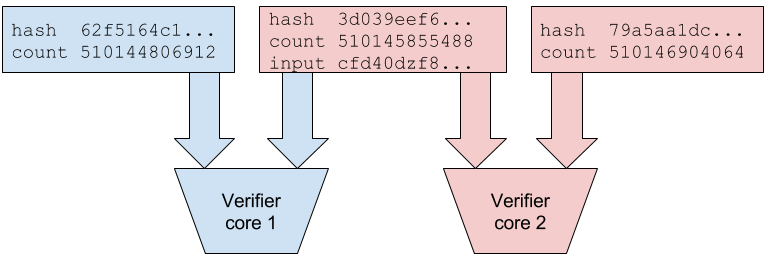
\includegraphics[width=0.9\textwidth]{figures/fig_4.png}
    \caption[Figure 4]{Verifica usando più core\label{fig:poh_verify}}
  \end{center}
  \end{figure}

Nell'esempio in Figura~\ref{fig:poh_verify}, ogni nucleo è in grado di verificare ogni sezione della sequenza in parallelo. Poiché tutte le stringhe di ingresso vengono registrate nell'uscita, con il contatore e lo stato in cui sono aggiunte, i verificatori possono replicare ogni striscia in parallelo. Gli hash di colore rosso indicano che la sequenza è stata modificata mediante l'inserimento di dati.

\subsection{Scaling Orizzontale}\label{poh:scale}
È possibile sincronizzare più generatori Proof of History mescolando lo stato di sequenza da un generatore all'altro e ottenendo così lo scaling orizzontale del generatore Proof of History. Questo scaling è fatto senza sharding. È necessaria l'uscita di entrambi i generatori  per ricostruire l'intero ordine degli eventi nel sistema.

\begin{center}
  \begin{tabular}{|l c r|}

  \hline
    \multicolumn{3}{|c|}{PoH Generator A} \\
  %  \hline
    Index & Hash & Data \\ \hline
    $1$ & \texttt{hash1a} & \\
    $2$ & \texttt{hash2a} & \texttt{hash1b} \\
    $3$ & \texttt{hash3a} & \\
    $4$ & \texttt{hash4a} & \\
    \hline
    \end{tabular}
  \begin{tabular}{| l  c  r |}
  \hline
    \multicolumn{3}{|c|}{PoH Generator B} \\
%    \hline
    Index & Hash & Data \\ \hline
    $1$ & \texttt{hash1b} & \\
    $2$ & \texttt{hash2b} & \texttt{hash1a} \\
    $3$ & \texttt{hash3b} & \\
    $4$ & \texttt{hash4b} & \\
    \hline
    \end{tabular}
\end{center}

Dati i generatori A e B, A riceve un pacchetto di dati da B (hash1b), che contiene l'ultimo stato dal generatore B, e l'ultimo stato dal generatore B osservato dal generatore A. L'hash di stato successivo nel generatore A dipende quindi dallo stato dal generatore B, quindi possiamo dedurre che hash1b è successo qualche tempo prima di hash3a. Questa proprietà è transitiva, quindi se tre generatori sono sincronizzati tramite un unico generatore comune \(A \leftrightarrow B \leftrightarrow C\), possiamo tracciare la dipendenza tra A e C anche se non sono stati sincronizzati direttamente.

Sincronizzando periodicamente i generatori, ogni generatore può quindi gestire una parte del traffico esterno, in modo che il sistema complessivo possa gestire una maggiore quantità di eventi da monitorare che dipende dall'accuratezza del tempo reale, a causa di latenze di rete tra i generatori. Un ordine globale può ancora essere raggiunto selezionando una funzione deterministica per ordinare qualsiasi evento che si trovi all'interno della finestra di sincronizzazione, come ad esempio il valore dell'hash stesso.


\begin{figure}
  \begin{center}
    \centering
    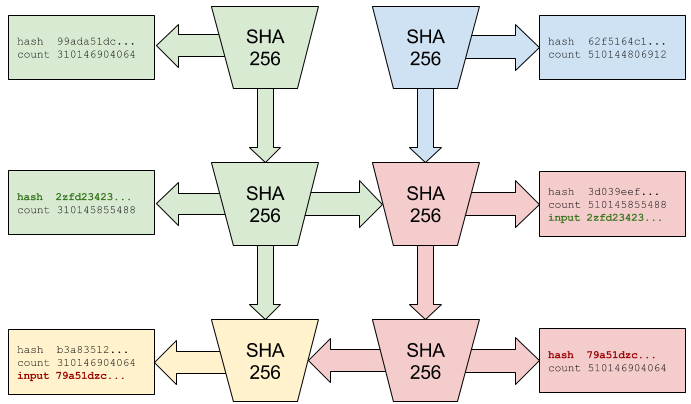
\includegraphics[width=0.9\textwidth]{figures/fig_5.png}
    \caption[Fig 5]{Sincronizzazione di due generatori\label{fig:poh_scale}}
  \end{center}
  \end{figure}

Nella Figura~\ref{fig:poh_scale}, i due generatori inseriscono lo stato di uscita dell'altro e registrano l'operazione. Il cambio di colore indica che i dati del peer hanno modificato la sequenza.  Le hash generate che vengono mixate in ciascun flusso sono evidenziate in grassetto. 

La sincronizzazione ha proprietà transitiva. \(A \leftrightarrow B \leftrightarrow C\). Esiste un ordine dimostrabile di eventi tra A e C attraverso B.

%%It is worth noting that the theoretical $710$k tx/s on a $1$~gb network based on the PoH design does not account for additional capacity offered through  horizontal scaling.
Questo tipo di scaling è limitato dalla Disponibilità. Connessioni da $10 \times 1$~gbps con disponibilità di 0,999 avrebbero disponibilità \(0,999^{10} = 0,99 \).

\subsection{Consistenza}
Gli utenti devono essere in grado di imporre la coerenza della sequenza generata e renderla resistente agli attacchi inserendo l'ultimo output osservato della sequenza che considerano valida nel loro input.\\

\begin{center}
  \begin{tabular}{ | l c r |}
    \hline
    \multicolumn{3}{|c|}{PoH Sequence A} \\
    Index & Data & Output Hash  \\ \hline
    $10$ & & \texttt{hash10a} \\
    $20$ & Event1 & \texttt{hash20a} \\
    $30$ & Event2 & \texttt{hash30a} \\
    $40$ & Event3 & \texttt{hash40a} \\
    \hline
    \end{tabular}
  \begin{tabular}{ | l c r |}
    \hline
    \multicolumn{3}{|c|}{PoH Hidden Sequence B} \\
    Index & Data & Output Hash \\ \hline
    $10$ & & \texttt{hash10b}\\
    $20$ & Event3 & \texttt{hash20b}  \\
    $30$ & Event2 & \texttt{hash30b} \\
    $40$ & Event1 & \texttt{hash40b} \\
    \hline
    \end{tabular}
\end{center}

Se un generatore di PoH dannoso ha accesso a tutti gli eventi contemporaneamente è in grado di generare una sequenza nascosta più rapida oppure può produrre una seconda sequenza nascosta con gli eventi in ordine inverso.\\

Per prevenire questo attacco, ogni Evento generato dal client dovrebbe contenere in sé l'ultimo hash che il client ha osservato da quella che considera una sequenza valida. Quindi, quando un client crea i dati "Event1", dovrebbe aggiungere l'ultimo hash che ha osservato.\\

\begin{center}
  \begin{tabular}{  l  c l}

    \multicolumn{3}{c}{PoH Sequence A} \\
    \hline
    Index  & Data & Output Hash  \\ \hline
    $10$ & & \texttt{hash10a} \\
    $20$ & Event1 = append(event1 data, \texttt{hash10a}) & \texttt{hash20a}  \\
    $30$ & Event2 = append(event2 data, \texttt{hash20a}) & \texttt{hash30a} \\
    $40$ &  Event3 = append(event3 data, \texttt{hash30a}) & \texttt{hash40a} \\
    \end{tabular}
\end{center}

Quando la sequenza viene pubblicata, Event3 fa riferimento a hash30a, e se non è nella sequenza precedente a questo Evento, gli utenti della sequenza sanno che è una sequenza non valida. L'attacco parziale di riordino sarebbe quindi limitato al numero di hash prodotti dal momento in cui il client ha osservato un evento a quando l'evento è stato inserito. I client dovrebbero quindi essere in grado di scrivere software senza presumere che l'ordine sia corretto per il breve periodo di hash tra l'ultimo hash osservato e quello inserito.

Per evitare che un generatore di PoH dannoso riscriva le hash dell'evento del client, i client possono inviare una firma dei dati dell'evento e l'ultimo hash osservato al posto dei soli dati.\\
\begin{center}
  \begin{tabular}{  l  l  r }
    \multicolumn{3}{c}{PoH Sequence A} \\
    \hline
    Index & Data & Output Hash \\ \hline
    $10$ & & hash10a  \\
    $20$ & \makecell{Event1 = sign(append(event1 data, hash10a), \\Client Private Key)} & hash20a\\
    $30$ & \makecell{Event2 = sign(append(event2 data, hash20a), \\Client Private Key)} & hash30a \\
    $40$ & \makecell{Event3 = sign(append(event3 data, hash30a), \\Client Private Key)} & hash40a \\

    \end{tabular}
\end{center}

La verifica di questi dati richiede una verifica della firma e una ricerca dell'hash nella sequenza di hash precedenti a questo..\\
\noindent Verifica:\\

\noindent\texttt{(Signature, PublicKey, hash30a, event3 data) = Event3} \\
\texttt{Verify(Signature, PublicKey, Event3)} \\
\texttt{Lookup(hash30a, PoHSequence)} \\

\begin{figure}
  \begin{center}
    \centering
    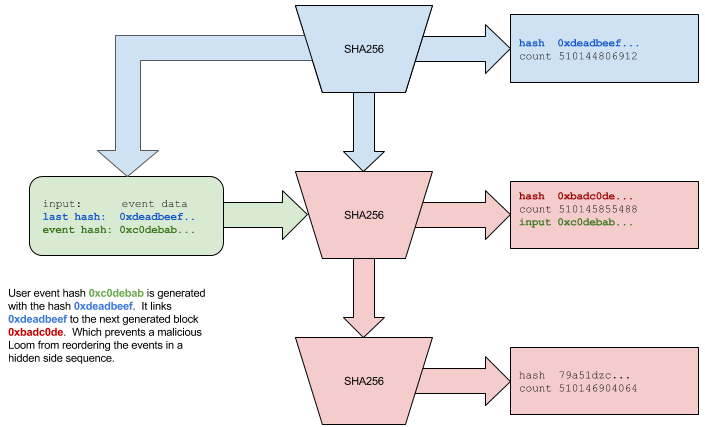
\includegraphics[width=0.9\textwidth]{figures/fig_6.png}
    \caption[Fig 6]{Input con retro riferimento.\label{fig:poh_consistency}}
  \end{center}
  \end{figure}

In Figura~\ref{fig:poh_consistency}, l'input fornito dall'utente dipende dall'hash \texttt{0xdeadbeef\ldots} esistente nella sequenza generata prima che l'hash fosse inserito. La freccia blu in alto a sinistra indica che il client sta facendo riferimento a un hash prodotto in precedenza. Il messaggio del client è valido solo in una sequenza che contiene l'hash \texttt{0xdeadbeef\ldots}. Il colore rosso nella sequenza indica che la sequenza è stata modificata dai dati del client	.

\subsection{Generalità}
4000 hash al secondo genererebbero 160 kilobytes addizionali di dati e avrebbero bisogno di una GPU con 4000 core e circa 0.25-0.75 millisecondi per la verifica.

\subsection{Attacchi}
\subsubsection{Reversal}
 Per generare un ordine inverso è necessario che l'aggressore avvii la sequenza dannosa dopo il secondo evento. Questo ritardo dovrebbe consentire a qualsiasi nodo peer to peer non dannoso di comunicare l'ordine originale.
 
\subsubsection{Velocità}
Avere più generatori può rendere l'implementazione più resistente agli attacchi. Un generatore potrebbe essere ad alta bandwidth 
e potrebbe ricevere molti eventi da mixare nella sua sequenza, un altro generatore potrebbe essere ad alta velocità e bassa bandwidth e potrebbe mescolarsi periodicamente con il generatore di alta larghezza di banda.

La sequenza ad alta velocità creerebbe una sequenza secondaria di dati che un attaccante dovrebbe invertire.

\subsubsection{Attacchi a lungo raggio}

Gli attacchi a lungo raggio comportano l'acquisizione di vecchie chiavi private client dismesse e la generazione di un registro falsificato ~\cite{casper}. La prova storica fornisce una certa protezione contro gli attacchi a lungo raggio. Un utente malintenzionato che ottiene l'accesso a vecchie chiavi private dovrebbe ricreare un record storico che richiede tanto tempo quanto quello originale che sta cercando di falsificare. Ciò richiederebbe l'accesso a un processore più veloce di quello attualmente in uso nella rete, altrimenti l'aggressore non potrebbe mai  raggiungere la lunghezza del record originale! 

Inoltre, un'unica fonte di tempo consente di costruire una prova di riproduzione più semplice (per saperne di più, si veda la Sezione~\ref{porep}). Poiché la rete è progettata in modo che tutti i partecipanti alla rete si basino su un'unica registrazione storica degli eventi.

PoRep e PoH insieme dovrebbero fornire una difesa di spazio e tempo contro un registro falsificato.


\section{Proof of Stake Consensus}\label{proof_of_stake}
\subsection{Descrizione}
This specific instance of Proof of Stake is designed for quick confirmation of the current sequence produced by the Proof of History generator, for voting and selecting the next Proof of History generator, and for punishing any misbehaving validators. This algorithm depends on messages eventually arriving to all participating nodes within a certain timeout.
\subsection{Terminology}
\begin{description}

\item[bonds]
Bonds are equivalent to a capital expense in Proof of Work. A miner buys hardware and electricity, and commits it to a single branch in a Proof of Work blockchain. A bond is coin that the validator commits as collateral while they are validating transactions.

\item[slashing]

The proposed solution to the nothing at stake problem in Proof of Stake systems~\cite{slasher}. When a proof of voting for a different branch is published, that branch can destroy the validator’s bond. This is an economic incentive designed to discourage validators from confirming multiple branches.
\item[super majority]
A super majority is \(\frac{2}{3}\)rds of the validators weighted by their bonds. A super majority vote indicates that the network has reached consensus, and at least \(\frac{1}{3}\)rd of the network would have had to vote maliciously for this branch to be invalid. This would put the economic cost of an attack at \(\frac{1}{3}\)rd of the market cap of the coin.

\end{description}

\subsection{Bonding}
A bonding transaction takes a \hyphenation{user specified} amount of coin and moves it to a bonding account under the user’s identity. Coins in the bonding account cannot be spent and have to remain in the account until the user removes them. The user can only remove stale coins that have timed out. Bonds are valid after super majority of the current stakeholders have confirmed the sequence.

\subsection{Voting}
It is anticipated that the Proof of History generator will be able to publish a signature of the state at a predefined period. Each bonded identity must confirm that signature by publishing their own signed signature of the state. The vote is a simple yes vote, without a no. If super majority of the bonded identities have voted within a timeout, then this branch would be accepted as valid.

\subsection{Unbonding}

Missing N number of votes marks the coins as stale and no longer eligible for voting. The user can issue an unbonding transaction to remove them.

N is a dynamic value based on the ratio of stale to active votes. N increases as the number of stale votes increases. In an event of a large network partition, this allows the larger branch to recover faster than the smaller branch.

\subsection{Elections}\label{subsec:elections}
Election for a new PoH generator occur when the PoH generator failure is detected. The validator with the largest voting power, or highest public key address if there is a tie is picked as the new PoH generator.

A super majority of confirmations are required on the new sequence. If the new leader fails before a super majority confirmations are available, the next highest validator is selected, and a new set of confirmations is required.

To switch votes, a validator needs to vote at a higher PoH sequence counter, and the new vote needs to contain the votes it wants to switch. Otherwise the second vote will be slashable. Vote switching is expected to be designed so that it can only occur at a height that does not have a super majority.

Once a PoH generator is established, a Secondary can be elected to take over the transactional processing duties. If a Secondary exists, it will be considered as the next leader during a Primary failure.

The platform is designed so that the Secondary becomes Primary and lower rank generators are promoted if an exception is detected or on a predefined schedule.
\subsection{Election Triggers}
\subsubsection{Forked Proof of History generator}

PoH generators are designed with an identity that signs the generated sequence. A fork can only occur in case the PoH generator’s identity has been compromised. A fork is detected because two different historical records have been published on the same PoH identity.

\subsubsection{Runtime Exceptions}
A hardware failure or a bug, or a intentional error in the PoH generator could cause it to generate an invalid state and publish a signature of the state that does not match the local validator’s result. Validators will publish the correct signature via gossip and this event would trigger a new round of elections. Any validators who accept an invalid state will have their bonds slashed.

\subsubsection{Network Timeouts}

A network timeout would trigger an election.

\subsection{Slashing}
Slashing occurs when a validator votes two separate sequences. A proof of malicious vote will remove the bonded coins from circulation and add them to the mining pool.

A vote that includes a previous vote on a contending sequence is not eligible as proof of malicious voting. Instead of slashing the bonds, this vote removes the currently cast vote on the contending sequence.

Slashing also occurs if a vote is cast for an invalid hash generated by the PoH generator. The generator is expected to randomly generate an invalid state, which would trigger a fallback to Secondary.
\subsection{Secondary Elections}
Secondary and lower ranked Proof of History generators can be proposed and approved. A proposal is cast on the primary generator’s sequence. The proposal contains a timeout, if the motion is approved by a super majority of the vote before the timeout, the Secondary is considered elected, and will take over duties as scheduled. Primary can do a soft handover to Secondary by inserting a message into the generated sequence indicating that a handover will occur, or inserting an invalid state and forcing the network to fallback to Secondary.

If a Secondary is elected, and the primary fails, the Secondary will be considered as the first fallback during an election.

\subsection{Availability}\label{availability}
CAP systems that deal with partitions have to pick Consistency or Availability. Our approach eventually picks Availability, but because we have an objective measure of time, Consistency is picked with reasonable human timeouts.

Proof of Stake verifiers lock up some amount of coin in a “stake”, which allows them to vote for a particular set of transactions. Locking up coin is a transaction that is entered into a PoH stream, just like any other transaction. To vote, a PoS verifier has to sign the hash of the state, as it was computed after processing all the transactions to a specific position in the PoH ledger. This vote is also entered as a transaction into the PoH stream. Looking at the PoH ledger, we can then infer how much time passed between each vote, and if a partition occurs, for how long each verifier has been unavailable.

To deal with partitions with reasonable human timeframes, we propose a dynamic approach to “unstake” unavailable verifiers. When the number of verifiers is high and above \(\frac{2}{3}\), the “unstaking” process can be fast. The number of hashes that must be generated into the ledger is low before the unavailable verifiers stake is fully unstaked and they are no longer counted for consensus. When the number of verifiers is below \(\frac{2}{3}\)rds but above \(\frac{1}{2}\), the unstaking timer is slower, requiring a larger number of hashes to be generated before the missing verifiers are unstaked. In a large partition, like a partition that is missing \(\frac{1}{2}\) or more of the verifiers, the unstaking process is very very slow. Transactions can still be entered into the stream, and verifiers can still vote, but full \(\frac{2}{3}\)rds consensus will not be achieved until a very large amount of hashes have been generated and the unavailable verifiers have been unstaked. The difference in time for a network to regain liveness allows us as customers of the network human timeframes to pick a partition that we want to continue using.

\subsection{Recovery}\label{availability}
In the system we propose, the ledger can be fully recovered from any failure. That means, anyone in the world can pick any random spot in the ledger and create a valid fork by appending newly generated hashes and transactions. If all the verifiers are missing from this fork, it would take a very very long time for any additional bonds to become valid and for this branch to achieve \(\frac{2}{3}\)rds super majority consensus. So full recovery with zero available validators would require a very large amount of hashes to be appended to the ledger, and only after all the unavailable validators have been unstaked will any new bonds be able to validate the ledger.

\subsection{Finality}\label{availability}
PoH allows verifiers of the network to observe what happened in the past with some degree of certainty of the time of those events. As the PoH generator is producing a stream of messages, all the verifiers are required to submit their signatures of the state within 500ms. This number can be reduced further depending on network conditions. Since each verification is entered into the stream, everyone in the network can validate that every verifier submitted their votes within the required timeout without actually observing the voting directly.

\subsection{Attacks}
\subsubsection{Tragedy of Commons}
The PoS verifiers simply confirm the state hash generated by the PoH generator. There is an economic incentive for them to do no work and simply approve every generated state hash. To avoid this condition, the PoH generator should inject an invalid hash at a random interval. Any voters for this hash should be slashed. When the hash is generated, the network should immediately promote the Secondary elected PoH generator.

Each verifier is required to respond within a small timeout - 500ms for example. The timeout should be set low enough that a malicious verifier has a low probability of observing another verifiers vote and getting their votes into the stream fast enough.

\subsubsection{Collusion with the PoH generator}\label{subsubsec:collusion}
A verifier that is colluding with the PoH generator would know in advance when the invalid hash is going to be produced and not vote for it. This scenario is really no different than the PoH identity having a larger verifier stake. The PoH generator still has to do all the work to produce the state hash.

\subsubsection{Censorship}\label{censorship}
Censorship or denial of service could occur when a \(\frac{1}{3}\)rd of the bond holders refuse to validate any sequences with new bonds. The protocol can defend against this form of attack by dynamically adjusting how fast bonds become stale. In the event of a denial of service, the larger partition will be designed to fork and censor the Byzantine bond holders. The larger network will recover as the Byzantine bonds become stale with time. The smaller Byzantine partition would not be able to move forward for a longer period of time.

The algorithm would work as follows. A majority of the network would elect a new Leader. The Leader would then censor the Byzantine bond holders from participating. Proof of History generator would have to continue generating a sequence, to prove the passage of time, until enough Byzantine bonds have become stale so the bigger network has a super majority. The rate at which bonds become stale would be dynamically based on what percentage of bonds are active. So the Byzantine minority fork of the network would have to wait much longer than the majority fork to recover a super majority. Once a super majority has been established, slashing could be used to permanently punish the Byzantine bond holders.

\subsubsection{Long Range Attacks}\label{censorship}
PoH provides a natural defense against long range attacks. Recovering the ledger from any point in the past would require the attacker to overtake the valid ledger in time by outpacing the speed of the PoH generator.

The consensus protocol provides a second layer of defense, as any attack would have to take longer than the time it takes to unstake all the valid validators. It also creates an availability “gap” in the history of the ledger. When comparing two ledgers of the same height, the one with the smallest maximum partition can be objectively considered as valid.

\subsubsection{ASIC Attacks}\label{censorship}

Two opportunities for ASIC attacks exist in this protocol - during partition, and cheating timeouts in Finality.

For ASIC attacks during Partitions, the Rate at which bonds are unstaked is non-linear, and for networks with large partitions the rate is orders of magnitude slower than expected gains from an ASIC attack.

For ASIC attacks during Finality, the vulnerability allows for byzantine validators who have a bonded stake to wait for confirmations from other nodes and inject their votes with a collaborating PoH generator. The PoH generator can then use its faster ASIC to generate 500ms worth of hashes in less time, and allow for network communication between PoH generator and the collaborating nodes. But, if the PoH generator is also byzantine, there is no reason why the byzantine generator wouldn’t have communicated the exact counter when they expect to insert the failure. This scenario is no different than a PoH generator and all the collaborators sharing the same identity vs. having a single combined stake and only using 1 set of hardware.

\section{Streaming Proof of Replication}\label{porep}
\subsection{Description}
Filecoin proposed a version of Proof of Replication \cite{filecoinporep}. The goal of this version is to have fast and streaming verifications of Proof of Replication, which are enabled by keeping track of time in a Proof of History generated sequence. Replication is not used as a consensus algorithm, but is a useful tool to account for the cost of storing the blockchain history or state at a high availability.
\subsection{Algorithm}
As shown in Figure~\ref{fig:encrypt} CBC encryption encrypts each block of data in sequence, using the previously encrypted block to XOR the input data.

\begin{figure}[h]
  \begin{center}
    \centering
    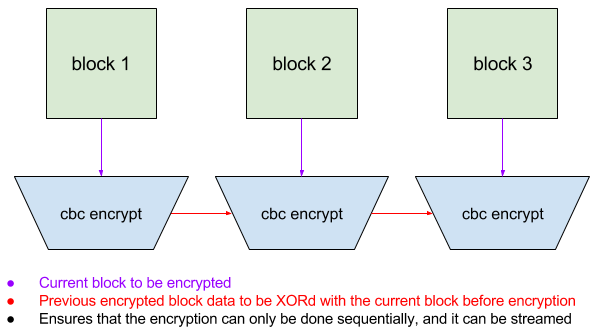
\includegraphics[width=0.9\textwidth]{figures/cbc_encryption_001.png}
    \caption[Fig 7]{Sequential CBC encryption\label{fig:encrypt}}
  \end{center}
  \end{figure}

Each replication identity generates a key by signing a hash that has been generated via a Proof of History sequence. This ties the key to a replicator’s identity, and to a specific Proof of History sequence. Only specific hashes can be selected. (See Section~\ref{hashselection} on Hash Selection)

The data set is fully encrypted block by block. Then to generate a proof, the key is used to seed a pseudorandom number generator that selects a random 32 bytes from each block.

A merkle hash is computed with the selected PoH hash prepended to the each slice.

\begin{figure}[h]
  \begin{center}
    \centering
    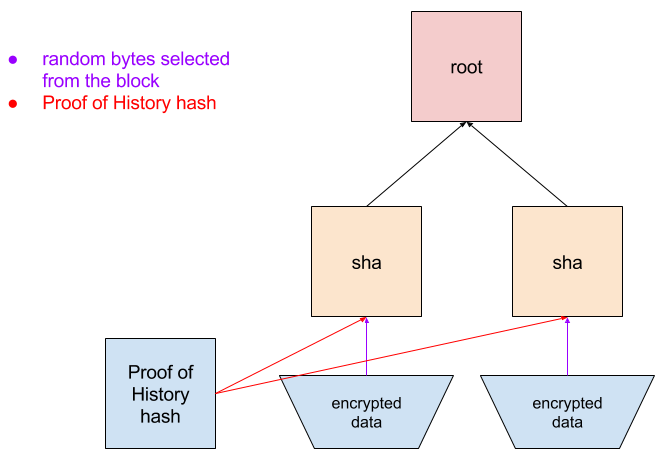
\includegraphics[width=0.9\textwidth]{figures/por_001.png}
    \caption[Fig 8]{Fast Proof of Replication\label{fig_8}}
  \end{center}
  \end{figure}

The root is published, along with the key, and the selected hash that was generated. The replication node is required to publish another proof in N hashes as they are generated by Proof of History generator, where N is approximately \(\frac{1}{2}\) the time it takes to encrypt the data. The Proof of History generator will publish specific hashes for Proof of Replication at predefined periods. The replicator node must select the next published hash for generating the proof. Again, the hash is signed, and random slices are selected from the blocks to create the merkle root.

After a period of N proofs, the data is re-encrypted with a new CBC key.
\subsection{Verification}

With N cores, each core can stream encryption for each identity. Total space required is \(2 blocks * N cores\), since the previous encrypted block is necessary to generate the next one. Each core can then be used to generate all the proofs that were derived from the current encrypted block.

Total time to verify proofs is expected to be equal to the time it takes to encrypt. The proofs themselves consume few random bytes from the block, so the amount of data to hash is significantly lower than the encrypted block size. The number of replication identities that can be verified at the same time is equal to the number of available cores. Modern GPUs have 3500+ cores available to them, albeit at \(\frac{1}{2}\)-\(\frac{1}{3}\) the clock speed of a CPU.

\subsection{Key Rotation}

Without key rotation the same encrypted replication can generate cheap proofs for multiple Proof of History sequences. Keys are rotated periodically and each replication is re-encrypted with a new key that is tied to a unique Proof of History sequence.

Rotation needs to be slow enough that it’s practical to verify replication proofs on GPU hardware, which is slower per core than CPUs.

\subsection{Hash Selection}\label{hashselection}

The Proof of History generator publishes a hash to be used by the entire network for encrypting Proofs of Replication, and for using as the pseudorandom number generator for byte selection in fast proofs.

The hash is published at a periodic counter that is roughly equal to \(\frac{1}{2}\) the time it takes to encrypt the data set. Each replication identity must use the same hash, and use the signed result of the hash as the seed for byte selection, or the encryption key.

The period that each replicator must provide a proof must be smaller than the encryption time. Otherwise the replicator can stream the encryption and delete it for each proof.

A malicious generator could inject data into the sequence prior to this hash to generate a specific hash. This attack is discussed more in \ref{subsubsec:collusion}.

\subsection{Proof Validation}
The Proof of History node is not expected to validate the submitted Proof of Replication proofs. It is expected to keep track of the number of pending and verified proofs submitted by the replicator’s identity. A proof is expected to be verified when the replicator is able to sign the proof by a super majority of the validators in the network.

The verifications are collected by the replicator via p2p gossip network, and submitted as one packet that contains a super majority of the validators in the network. This packet verifies all the proofs prior to a specific hash generated by the Proof of History sequence, and can contain multiple replicator identities at once.
\subsection{Attacks}
\subsubsection{Spam}
A malicious user could create many replicator identities and spam the network with bad proofs. To facilitate faster verification, nodes are required to provide the encrypted data and the entire merkle tree to the rest of the network when they request verification.

The Proof of Replication that is designed in this paper allows for cheap verification of any additional proofs, as they take no additional space. But each identity would consume 1 core of encryption time. The replication target should be set to a maximum size of readily available cores. Modern GPUs ship with 3500+ cores.

\subsubsection{Partial Erasure}

A replicator node could attempt to partially erase some of the data to avoid storing the entire state. The number of proofs and the randomness of the seed should make this attack difficult.

For example, a user storing 1 terabyte of data erases a single byte from each 1 megabyte block. A single proof that samples 1 byte out of every megabyte would have a likelihood of collision with any erased byte \(1 - (1- 1/1,000,0000)^{1,000,000} = 0.63\). After 5 proofs the likelihood is \(0.99\).

\subsubsection{Collusion with PoH generator}

The signed hash is expected to be used to seed the sample. If a replicator could select a specific hash in advance then the replicator could erase all bytes that are not going to be sampled.

A replicator identity that is colluding with the Proof of History generator could inject a specific transaction at the end of the sequence before the predefined hash for random byte selection is generated. With enough cores, an attacker could generate a hash that is preferable to the replicator’s identity.

This attack could only benefit a single replicator identity. Since all the identities have to use the same exact hash that is cryptographically signed with ECDSA (or equivalent), the resulting signature is unique for each replicator identity, and collision resistant. A single replicator identity would only have marginal gains.
\subsubsection{Denial of Service}
The cost of adding an additional replicator identity is expected to be equal to the cost of storage. The cost of adding extra computational capacity to verify all the replicator identities is expected to be equal to the cost of a CPU or GPU core per replication identity.

This creates an opportunity for a denial of service attack on the network by creating a large number of valid replicator identities.

To limit this attack, the consensus protocol chosen for the network can select a replication target, and award the replication proofs that meet the desired characteristics, like availability on the network, bandwidth, geolocation etc...
\subsubsection{Tragedy of Commons}

The PoS verifiers could simply confirm PoRep without doing any work. The economic incentives should be lined up with the PoS verifiers to do work, i.e. splitting the mining payout between the PoS verifiers and the PoRep replication nodes.

To further avoid this scenario, the PoRep verifiers can submit false proofs a small percentage of the time. They can prove the proof is false by providing the function that generated the false data. Any PoS verifier that confirmed a false proof would be slashed.

\section{System Architecture}\label{system_architecture}

\begin{figure}
  \begin{center}
    \centering
    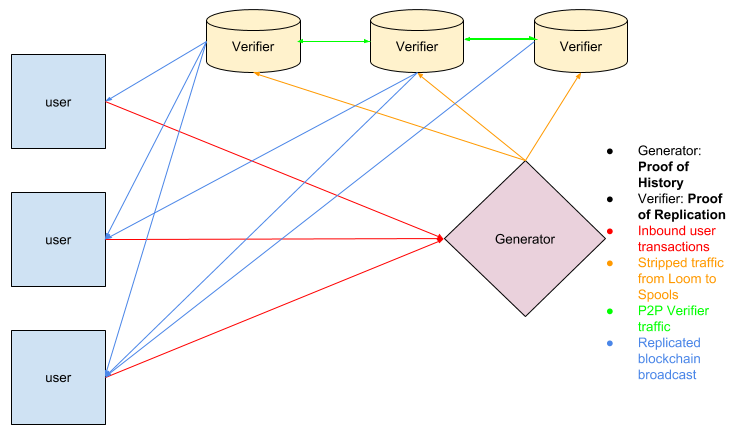
\includegraphics[width=0.9\textwidth]{figures/system_arch_001.png}
    \caption[Fig 9]{System Architecture \label{fig_9}}
  \end{center}
  \end{figure}

\subsection{Components}

\subsubsection{Leader, Proof of History generator}
The Leader is an elected Proof of History generator. It consumes arbitrary user transactions and outputs a Proof of History sequence of all the transactions that guarantee a unique global order in the system. After each batch of transactions the Leader outputs a signature of the state that is the result of running the transactions in that order. This signature is signed with the identity of the Leader.

\subsubsection{State}
The state is a naive hash table indexed by the user’s address. Each cell contains the full user’s address and the memory required for this computation. For example,\\
\noindent the Transaction table contains:\\\\\noindent
\begin{bytefield}[bitwidth=.1em]{256}
\bitheader{0,31,63,95,127,159,191,223,255} \\
\bitbox{160}{Ripemd of Users Public Key}
& \bitbox{64}{Account}
& \bitbox{32}{unused}
\end{bytefield}\\
for a total of 32 bytes.\\
\noindent The Proof of Stake bond’s table contains:\\\\\noindent
\begin{bytefield}[bitwidth=.1em]{256}
\bitheader{0,31,63,95,127,159,191,223,255} \\
\bitbox{160}{Ripemd of Users Public Key}
& \bitbox{64}{Bond} \\
& \bitbox{64}{Last Vote} \\
& \bitbox{224}{unused}
\end{bytefield}\\
for a total of 64 bytes.
\subsubsection{Verifier, State Replication}



The Verifier nodes replicate and provide high availability of the blockchain state. The replication target is selected by the consensus algorithm, and the validators in the consensus algorithm select and vote the Proof of Replication nodes they approve of based on off-chain defined criteria.


The network could be configured with a minimum Proof of Stake bond size, and a requirement for a single replicator identity per bond.
\subsubsection{Validators}
These nodes are consuming bandwidth from Verifiers. They are virtual nodes, and can run on the same machines as the Verifiers or the Leader, or on separate machines that are specific to the consensus algorithm configured for this network.

\subsection{Network Limits}

\begin{figure}
  \begin{center}
    \centering
    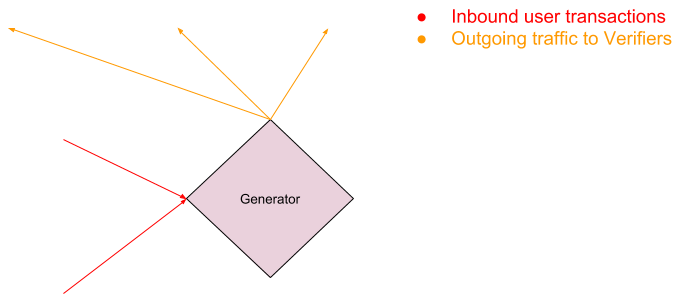
\includegraphics[width=0.8\textwidth]{figures/generator_network_limits_001.png}
    \caption[Fig 10]{Generator network limits\label{fig_10}}
  \end{center}
  \end{figure}

The leader is expected to be able to take incoming user packets, order them in the most efficient way possible, and sequence them into a Proof of History sequence that is published to downstream Verifiers. Efficiency is based on memory access patterns of the transactions, so the transactions are ordered to minimize faults and to maximize prefetching.\\\\

\noindent \textbf{Incoming packet format:}\\\\\noindent
\begin{bytefield}[bitwidth=.1em]{256}
\bitheader{0,31,63,95,127,159,191,223,255} \\
\begin{rightwordgroup}{Signed}
\bitbox{160}{Last Valid Hash}
& \bitbox{64}{Counter}
& \bitbox{6}{u}
& \bitbox{10}{s} \\
& \bitbox{64}{Fee} \\
& \bitbox{256}{From} \\
\end{rightwordgroup} \\
& \bitbox{256}{Signature 1 of 2} \\
& \bitbox{256}{Signature 2 of 2} \\
\end{bytefield}

\noindent Size \(20 + 8 + 16 + 8 + 32 + 32 + 32 = 148\) bytes.\\\\

The minimal payload that can be supported would be 1 destination account with a minimum size of 176 bytes.\\\\

\noindent \textbf{With payload:}\\\\\noindent

\begin{bytefield}[bitwidth=.1em]{256}
\bitheader{0,31,63,95,127,159,191,223,255} \\
\begin{rightwordgroup}{Signed}
\bitbox{160}{Last Valid Hash}
& \bitbox{64}{Counter}
& \bitbox{6}{u}
& \bitbox{10}{s} \\
& \bitbox{160}{To}
& \bitbox{64}{Amount} \\
& \bitbox{64}{Counter}
& \bitbox{64}{Fee} \\
& \bitbox{256}{From} \\
\end{rightwordgroup} \\
& \bitbox{256}{Signature 1 of 2} \\
& \bitbox{256}{Signature 2 of 2} \\
\end{bytefield}

\noindent With payload the minimum size: 176 bytes\\\\

The Proof of History sequence packet contains the current hash, counter, and the hash of all the new messages added to the PoH sequence and the state signature after processing all the messages. This packet is sent once every N messages are broadcast.\\
\noindent Proof of History packet:\\\\\noindent
\begin{bytefield}[bitwidth=.1em]{256}
\bitheader{0,31,63,95,127,159,191,223,255} \\
\begin{rightwordgroup}{Signed}
\bitbox{160}{Current Hash}
& \bitbox{64}{Counter} \\
\bitbox{160}{Messages Hash} \\
\bitbox{160}{State Hash} \\
\end{rightwordgroup} \\
& \bitbox{256}{Signature 1 of 2} \\
& \bitbox{256}{Signature 2 of 2} \\
\end{bytefield}

\noindent Minimum size of the output packet is: 132 bytes \\\\

On a 1gbps network connection the maximum number of transactions possible is $1$~gigabit per second / $176$~bytes = $710$k tps max. Some loss ($1-4\%$) is expected due to Ethernet framing. The spare capacity over the target amount for the network can be used to increase availability by coding the output with Reed-Solomon codes, and striping it to the available downstream Verifiers.
\subsection{Computational Limits}
Each transaction requires a digest verification. This operation does not use any memory outside of the transaction message itself and can be parallelized independently. Thus throughput is expected to be limited by the number of cores available on the system.

GPU based ECDSA verification servers have had experimental results of 900k operations per second~\cite{gpuecc}.
\subsection{Memory Limits}
A naive implementation of the state as a \(50\%\) full hashtable with 32 byte entries for each account, would theoretically fit 10 billion accounts into 640GB. Steady state random access to this table is measured at \(1.1 * 10^7\) writes or reads per second. Based on 2 reads and two writes per transaction, memory throughput can handle 2.75m transactions per second. This was measured on an Amazon Web Services 1TB x1.16xlarge instance.

\subsection{High Performance Smart Contracts}\label{sec:smartcontracts}

Smart contracts are a generalized form of transactions. These are programs that run on each node and modify the state. This design leverages extended Berkeley Packet Filter bytecode, which is fast and easy to analyze, and JIT bytecode as the smart contracts language.

One of its main advantages is a zero cost Foreign Function Interface. Intrinsics, or \hyphenation{high level} functions that are implemented on the platform directly, are callable by \hyphenation{user supplied} programs. Calling the intrinsics suspends that program and schedules the intrinsic on a high performance server. Intrinsics are batched together to execute in parallel on the GPU.

\begin{figure}
  \begin{center}
    \centering
    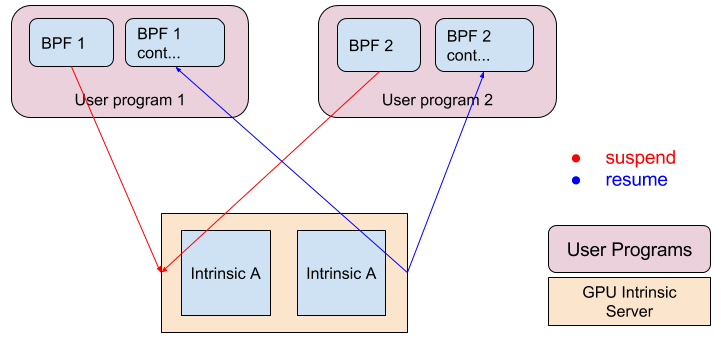
\includegraphics[width=0.9\textwidth]{figures/bpf_programs_001.png}
    \caption[Fig 11]{Executing \hyphenation{user supplied} BPF programs.\label{fig_11}}
  \end{center}
  \end{figure}

In the above example, two different user programs call the same intrinsic. Each program is suspended until the batch execution of the intrinsics is complete. An example intrinsic is ECDSA verification. Batching these calls to execute on the GPU can increase throughput by thousands of times.

This trampoline requires no native operating system thread context switches, since the BPF bytecode has a well defined context for all the memory that it is using.

eBPF backend has been included in LLVM since 2015, so any LLVM frontend language can be used to write smart contracts. It’s been in the Linux kernel since 2015, and the first iterations of the bytecode have been around since 1992. A single pass can check eBPF for correctness, ascertain its runtime and memory requirements and convert it to x86 instructions.

\bibliographystyle{abbrv}
\bibliography{simple}

\begin{thebibliography}{9}
\bibitem{liskov}
Liskov, Practical use of Clocks
\\\texttt{ http://www.dainf.cefetpr.br/~tacla/SDII/PracticalUseOfClocks.pdf}

\bibitem{spanner}
Google Spanner TrueTime consistency
\\\texttt{ https://cloud.google.com/spanner/docs/true-time-external-consistency}

\bibitem{ordering}
Solving Agreement with Ordering Oracles
\\\texttt{ http://www.inf.usi.ch/faculty/pedone/Paper/2002/2002EDCCb.pdf}

\bibitem{tendermint}
Tendermint: Consensus without Mining
\\\texttt{https://tendermint.com/static/docs/tendermint.pdf}

\bibitem{hashgraph}
Hedera: A Governing Council \& Public Hashgraph Network
\\\texttt{https://s3.amazonaws.com/hedera-hashgraph/hh-whitepaper-v1.0-180313.pdf}

\bibitem{filecoinporep}
Filecoin, proof of replication,
\\\texttt{https://filecoin.io/proof-of-replication.pdf}

\bibitem{slasher}
Slasher, A punative Proof of Stake algorithm
\\\texttt{https://blog.ethereum.org/2014/01/15/slasher-a-punitive-proof-of-stake-algorithm/}

\bibitem{delegatedpos}
BitShares Delegated Proof of Stake
\\\texttt{https://github.com/BitShares/bitshares/wiki/Delegated-Proof-of-Stake}

\bibitem{gpuecc}
An Efficient Elliptic Curve Cryptography Signature Server With GPU Acceleration
\\\texttt{http://ieeexplore.ieee.org/document/7555336/}

\bibitem{casper}
Casper the Friendly Finality Gadget
\\\texttt{https://arxiv.org/pdf/1710.09437.pdf}
\end{thebibliography}
\end{document}
This is never printed
